%% generato automaticamente da tools/build_tex.py --- non modificare
\chapter{Un operatore che confonde seno e coseno}
\label{cap:trasformata-t}
\quaderno{Trasformata T.dfw}{17 Jan 2011}{14}

Gennaio 2011, il quaderno più recente della raccolta. Quattordici righe, tutte della stessa forma, che applicano a quattordici funzioni diverse un unico operatore:
\[
  T[f](t)=\frac{\dfrac{1}{t}\displaystyle\int_0^t f(x)\,\mathrm{d}x}{f\!\left(\dfrac{t}{2}\right)}
\]
cioè il rapporto fra il valor medio di $f$ sull'intervallo $[0,t]$ e il valore che $f$ assume nel punto di mezzo. Se $f$ fosse una retta i due numeri coinciderebbero e il rapporto varrebbe uno; per tutte le altre funzioni il rapporto misura di quanto la funzione si scosta dalla propria corda.

\section{Le funzioni logaritmiche}

Le prime due righe applicano l'operatore ai logaritmi. Sono anche le uniche in cui il risultato resta ingombrante.

\begin{espr}{1}{User}{}
\begin{align*}
& \frac{\frac{1}{t}\, \int_{0}^{t} \ln\!\left(x + 1\right) \,\mathrm{d}x}{\ln\!\left(\frac{t}{2} + 1\right)} \\
=\;& \frac{\ln^{\frac{t + 1}{t}}\!\left(t + 1\right) - 1}{\ln\!\left(\frac{t}{2} + 1\right)}
\end{align*}
\end{espr}
Il logaritmo traslato. La potenza $(t+1)^{(t+1)/t}$ nasce dal raccogliere $\ln$ nel valor medio.

\begin{espr}{2}{User}{\verificata}
\begin{align*}
& \frac{\frac{1}{t}\, \int_{0}^{t} \ln\!\left(x\right) \,\mathrm{d}x}{\ln\!\left(\frac{t}{2}\right)} \\
=\;& \frac{\ln\!\left(t\right) - 1}{\ln\!\left(\frac{t}{2}\right)}
\end{align*}
\end{espr}
Il logaritmo semplice: il valor medio vale $\ln t-1$.


Il calcolo è diretto: $\int_0^t\ln(x+1)\,\mathrm{d}x=(t+1)\ln(t+1)-t$, e dividendo per $t$ si ottiene $\ln\!\left[(t+1)^{(t+1)/t}\right]-1$, che è esattamente il numeratore della riga $\#1$. Analogamente per il logaritmo semplice.

\section{Le funzioni circolari danno tutte lo stesso nucleo}

Qui sta il risultato del quaderno. Si applica l'operatore all'esponenziale, al seno, al coseno e all'esponenziale immaginario, e le risposte convergono.

\begin{espr}{3}{User}{\verificata}
\[
\frac{\frac{1}{t}\, \int_{0}^{t} \mathrm{e}^{x} \,\mathrm{d}x}{\mathrm{e}^{\frac{t}{2}}} = \frac{\sinh\!\left(\frac{t}{2}\right)}{\frac{t}{2}}
\]
\end{espr}
L'esponenziale reale dà il seno iperbolico cardinale.

\begin{espr}{4}{User}{\verificata}
\begin{align*}
& \frac{\frac{1}{t}\, \int_{0}^{t} \sin\!\left(x\right) \,\mathrm{d}x}{\sin\!\left(\frac{t}{2}\right)} \\
=\;& \frac{\sin\!\left(\frac{t}{2}\right)}{\frac{t}{2}}
\end{align*}
\end{espr}
Il seno dà il seno cardinale.

\begin{espr}{5}{User}{\verificata}
\begin{align*}
& \frac{\frac{1}{t}\, \int_{0}^{t} \cos\!\left(x\right) \,\mathrm{d}x}{\cos\!\left(\frac{t}{2}\right)} \\
=\;& \frac{\sin\!\left(\frac{t}{2}\right)}{\frac{t}{2}}
\end{align*}
\end{espr}
Il coseno dà lo stesso risultato del seno: l'operatore non li distingue.

\begin{espr}{6}{User}{\verificata}
\begin{align*}
& \frac{\frac{1}{t}\, \int_{0}^{t} \mathrm{e}^{\mathrm{i}\, x} \,\mathrm{d}x}{\mathrm{e}^{\frac{\mathrm{i}\, t}{2}}} \\
=\;& \frac{\sin\!\left(\frac{t}{2}\right)}{\frac{t}{2}}
\end{align*}
\end{espr}
E nemmeno l'esponenziale immaginario, che li contiene entrambi.

\begin{espr}{7}{User}{\verificata}
\begin{align*}
& \frac{\frac{1}{t}\, \int_{0}^{t} \mathrm{e}^{2\, \pi\, \mathrm{i}\, x} \,\mathrm{d}x}{\mathrm{e}^{\pi\, \mathrm{i}\, t}} \\
=\;& \frac{\sin\!\left(\pi\, t\right)}{\pi\, t}
\end{align*}
\end{espr}
Con pulsazione $2\pi$ il nucleo diventa $\sin(\pi t)/(\pi t)$: la forma normalizzata del seno cardinale.


Per il seno: $\int_0^t\sin x\,\mathrm{d}x=1-\cos t=2\sin^2\tfrac t2$, e dividendo per $t$ e per $\sin\tfrac t2$ resta $\dfrac{\sin(t/2)}{t/2}$. Per il coseno: $\int_0^t\cos x\,\mathrm{d}x=\sin t=2\sin\tfrac t2\cos\tfrac t2$, e dividendo per $t$ e per $\cos\tfrac t2$ resta di nuovo $\dfrac{\sin(t/2)}{t/2}$. L'operatore non distingue il seno dal coseno, e nemmeno dall'esponenziale immaginario che li contiene entrambi: tutti e tre danno il seno cardinale.

Per l'esponenziale reale il conto è lo stesso con le funzioni iperboliche e dà $\dfrac{\sinh(t/2)}{t/2}$: la stessa forma, con il seno sostituito dal suo analogo. Le due risposte sono l'una il prolungamento analitico dell'altra.

\section{Le potenze danno una costante}

Una riga sola, e con il risultato più sorprendente del gruppo.

\begin{espr}{8}{User}{\verificata}
\[
\frac{\frac{1}{t}\, \int_{0}^{t} x^{n} \,\mathrm{d}x}{\left(\frac{t}{2}\right)^{n}} = \frac{2^{n}}{n + 1}
\]
\end{espr}
Per le potenze il rapporto è costante: non dipende dall'ampiezza dell'intervallo ma solo dal grado.

\begin{figure}[htbp]
  \centering
  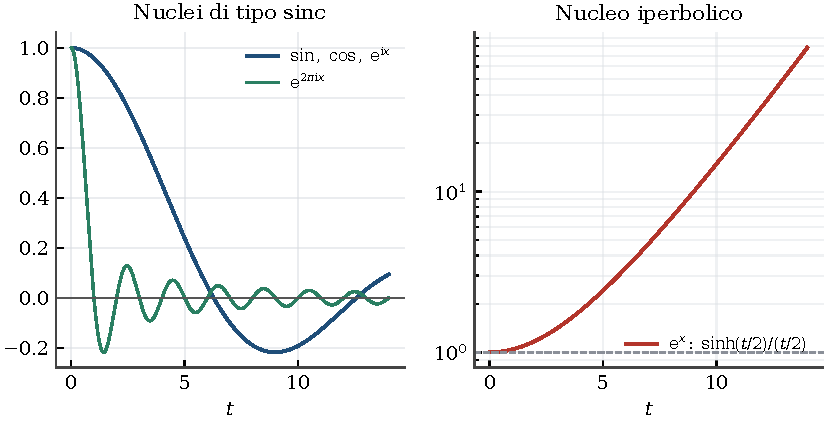
\includegraphics[width=0.86\linewidth]{../figures/trasformata_t.pdf}
  \caption{A sinistra il nucleo comune alle funzioni circolari, in due normalizzazioni. A destra il nucleo dell'esponenziale reale, in scala logaritmica: stessa formula, funzione iperbolica al posto di quella circolare, e crescita illimitata.}
  \label{fig:trasformata_t}
\end{figure}

Il rapporto non dipende da $t$: vale $2^n/(n+1)$ per ogni intervallo. Il motivo è l'omogeneità — sia il valor medio sia il valore nel punto di mezzo sono proporzionali a $t^n$, e il rapporto si semplifica.

Questa riga permette anche di riconoscere che cosa stia misurando l'operatore. Lo sviluppo di $T[f]$ per $t$ piccolo è
\[
  T[f](t)=1+\frac{t^2}{24}\,\frac{f''}{f}+O\!\left(t^4\right),
\]
che è l'errore relativo della formula di quadratura del punto medio. Per il seno $f''/f=-1$ e si ottiene $1-t^2/24$, che è lo sviluppo di $\mathrm{sinc}(t/2)$; per l'esponenziale $f''/f=+1$ e si ottiene $1+t^2/24$, cioè $\sinh(t/2)/(t/2)$; per $x^n$ valutato nel punto medio si ottiene $1+n(n-1)/6$, che coincide con $2^n/(n+1)$ per $n\le3$. L'operatore $T$, in altre parole, è l'errore della regola del punto medio scritto come funzione dell'ampiezza dell'intervallo.

\section{Le funzioni non elementari}

Le ultime sei righe applicano l'operatore a funzioni le cui primitive richiedono funzioni speciali o forme meno maneggevoli.

\begin{espr}{9}{User}{\verificata}
\begin{align*}
& \frac{\frac{1}{t}\, \int_{0}^{t} \mathrm{e}^{-x^{2}} \,\mathrm{d}x}{\mathrm{e}^{-\left(\frac{t}{2}\right)^{2}}} \\
=\;& \frac{\sqrt{\pi}\, \mathrm{e}^{\frac{t^{2}}{4}}\, \operatorname{erf}\!\left(t\right)}{2\, t}
\end{align*}
\end{espr}
La gaussiana introduce la funzione degli errori.

\begin{espr}{10}{User}{\verificata}
\begin{align*}
& \frac{\frac{1}{t}\, \int_{0}^{t} \frac{\sin\!\left(x\right)}{x} \,\mathrm{d}x}{\frac{\sin\!\left(\frac{t}{2}\right)}{\frac{t}{2}}} \\
=\;& \frac{\int_{0}^{t} \frac{\sin\!\left(x\right)}{x} \,\mathrm{d}x}{2\, \sin\!\left(\frac{t}{2}\right)}
\end{align*}
\end{espr}
L'operatore applicato al seno cardinale: il denominatore cancella il fattore $1/t$ e resta il seno integrale.

\begin{espr}{11}{User}{\verificata}
\begin{align*}
& \frac{\frac{1}{t}\, \int_{0}^{t} \arctan\!\left(x\right) \,\mathrm{d}x}{\arctan\!\left(\frac{t}{2}\right)} \\
=\;& \frac{\arctan\!\left(t\right) - \frac{\ln\!\left(t^{2} + 1\right)}{2\, t}}{\arctan\!\left(\frac{t}{2}\right)}
\end{align*}
\end{espr}
L'arcotangente: il valor medio è $\arctan t-\ln(1+t^2)/(2t)$.

\begin{espr}{12}{User}{\verificata}
\begin{align*}
& \frac{\frac{1}{t}\, \int_{0}^{t} \arcsin\!\left(x\right) \,\mathrm{d}x}{\arcsin\!\left(\frac{t}{2}\right)} \\
=\;& \frac{\arcsin\!\left(t\right) + \frac{\sqrt{1 - t^{2}} - 1}{t}}{\arcsin\!\left(\frac{t}{2}\right)}
\end{align*}
\end{espr}
L'arcoseno.

\begin{espr}{13}{User}{\verificata}
\begin{align*}
& \frac{\frac{1}{t}\, \int_{0}^{t} \arccos\!\left(x\right) \,\mathrm{d}x}{\arccos\!\left(\frac{t}{2}\right)} \\
=\;& -\frac{2\, t\, \arcsin\!\left(t\right) + 2\, \sqrt{1 - t^{2}} - \pi\, t - 2}{2\, t\, \arccos\!\left(\frac{t}{2}\right)}
\end{align*}
\end{espr}
L'arcocoseno, con la forma riordinata da Derive.

\begin{espr}{14}{User}{\verificata}
\begin{align*}
& \frac{\frac{1}{t}\, \int_{0}^{t} \tan\!\left(x\right) \,\mathrm{d}x}{\tan\!\left(\frac{t}{2}\right)} \\
=\;& \frac{-\ln\!\left(\cos\!\left(t\right)\right)\, \cot\!\left(\frac{t}{2}\right)}{t}
\end{align*}
\end{espr}
La tangente: il valor medio è $-\ln\cos t$ diviso $t$, e il risultato contiene la cotangente dell'angolo metà.


La riga $\#9$ è l'unica in cui compare una funzione speciale: il valor medio della gaussiana su $[0,t]$ è $\sqrt\pi\,\operatorname{erf}(t)/(2t)$, e dividendo per il valore nel punto medio $\mathrm{e}^{-t^2/4}$ si ottiene la forma scritta. La riga $\#10$ applica l'operatore al seno cardinale stesso, e il risultato si semplifica in modo notevole: il denominatore $\sin(t/2)/(t/2)$ cancella il fattore $1/t$ e resta il seno integrale diviso per $2\sin(t/2)$.

\section*{In sintesi}
\addcontentsline{toc}{section}{In sintesi}

Quattordici righe che dicono una cosa sola, ma la dicono bene: il rapporto fra la media di una funzione e il suo valore nel punto medio è una quantità che dipende quasi solo dalla curvatura. Per tutte le funzioni con $f''=-f$ dà il seno cardinale, per tutte quelle con $f''=+f$ il suo analogo iperbolico, per le potenze una costante. È l'ultimo quaderno della raccolta, ed è anche il più ordinato.

Il fatto ha un nome: è il caso unidimensionale del teorema della media per l'equazione di Helmholtz. Vale anche il viceversa: le funzioni per cui il rapporto fra la media su un intervallo e il valore nel suo centro dipende solo dall'ampiezza dell'intervallo sono esattamente le soluzioni di $f''=\lambda f$.

